\chapter{Introduction}
\label{chap: intro}
%\thispagestyle{empty}
\setcounter{page}{1}
\pagenumbering{arabic}


\vspace*{-2mm}
\section{Name of first section}
\label{sec: chap1 motivation}

\lipsum[9-13]


\section{Name of second section}
\label{sec: chap1 background}

\lipsum[14-18]

\subsection{Name of subsection}
\label{subsec: chap1 background2}

\renewcommand{\SF}{0.85}    % This 'scaling factor' is used to change the size of the image below without having to change the elements of the tikz picture
\begin{figure}[b]
    \centering
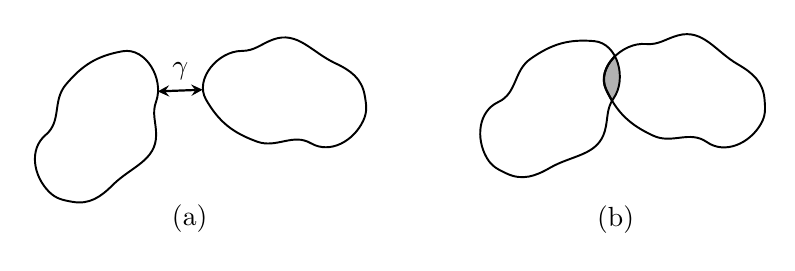
\begin{tikzpicture}[scale=\SF]
    \begin{scope}[scale=0.5]
        \draw[black,line width=0.7pt] (-1.2,1) to[out=50,in=190] (0.5,2) to[out=10,in=70] (1.5,0.5)
        to[out=-110,in=90] (1.5,-0.5) to[out=-90,in=45] (0.2,-2) to[out=-135,in=-10] (-1,-2.5) to[out=170,in=-45] (-1.7,-2.2) to[out=135,in=-140] (-1.8,-0.5) to[out=40,in=-130] (-1.2,1);
        \CoM{0}{0.1cm}{2mm};

        \draw[rotate=110,xshift=-1cm,yshift=-5cm,black,line width=0.7pt] (-1.2,1) to[out=50,in=190] (0.5,2) to[out=10,in=70] (1.5,0.5)
        to[out=-110,in=90] (1.5,-0.5) to[out=-90,in=45] (0.2,-2) to[out=-135,in=-10] (-1,-2.5) to[out=170,in=-45] (-1.7,-2.2) to[out=135,in=-140] (-1.8,-0.5) to[out=40,in=-130] (-1.2,1);
        \CoM{5.8cm}{0.5cm}{2mm};

        \draw[>=stealth,<->,thick] (1.55,0.8) -- node[pos=0.5,above]{\TS $\gamma$} (2.89,0.85);
        \draw (2.5,-3) node{\TS (a)};
    \end{scope}

    \begin{scope}[rotate=-15,scale=0.5,xshift=13cm,yshift=4cm]
        \begin{scope}
            \clip (-1.2,1) to[out=50,in=190] (0.5,2) to[out=10,in=70] (1.5,0.5)
        to[out=-110,in=90] (1.5,-0.5) to[out=-90,in=45] (0.2,-2) to[out=-135,in=-10] (-1,-2.5) to[out=170,in=-45] (-1.7,-2.2) to[out=135,in=-140] (-1.8,-0.5) to[out=40,in=-130] (-1.2,1);
            \filldraw[rotate=120,xshift=-0.5cm,yshift=-3.4cm,fill=black!30,draw=black,thick] (-1.2,1) to[out=50,in=190] (0.5,2) to[out=10,in=70] (1.5,0.5) to[out=-110,in=90] (1.5,-0.5) to[out=-90,in=45] (0.2,-2) to[out=-135,in=-10] (-1,-2.5) to[out=170,in=-45] (-1.7,-2.2) to[out=135,in=-140] (-1.8,-0.5) to[out=40,in=-130] (-1.2,1);
        \end{scope}

        \draw[black,line width=0.7pt] (-1.2,1) to[out=50,in=190] (0.5,2) to[out=10,in=70] (1.5,0.5)
        to[out=-110,in=90] (1.5,-0.5) to[out=-90,in=45] (0.2,-2) to[out=-135,in=-10] (-1,-2.5) to[out=170,in=-45] (-1.7,-2.2) to[out=135,in=-140] (-1.8,-0.5) to[out=40,in=-130] (-1.2,1);
        \CoM{0}{0.1cm}{2mm};

        \draw[rotate=120,xshift=-0.5cm,yshift=-3.4cm,black,line width=0.7pt] (-1.2,1) to[out=50,in=190] (0.5,2) to[out=10,in=70] (1.5,0.5)
        to[out=-110,in=90] (1.5,-0.5) to[out=-90,in=45] (0.2,-2) to[out=-135,in=-10] (-1,-2.5) to[out=170,in=-45] (-1.7,-2.2) to[out=135,in=-140] (-1.8,-0.5) to[out=40,in=-130] (-1.2,1);
        \CoM{4cm}{1cm}{2mm};

        \draw (2.5,-3) node{\TS (b)};
    \end{scope}
\end{tikzpicture}
\caption{This is the current style and layout of a figure caption.}
    \label{fig: chap1 impact bodies}
\end{figure}

\lipsum[19-23]


\subsection{Name of second subsection}
\label{subsec: chap1 background3}

\lipsum[1-5]

%\newpage
\section{Problem statement}
\label{sec: chap1 prob statement}

\lipsum[6-8]
Summarizing, the objective of the research is:
\vspace*{3mm}
\objective{State the objective of your PhD research here.}


\section{Research challenges and contributions}
\label{sec: chap1 contributions}

In this section, the research problem is divided in ... research challenges with the topics: topic 1, topic 2, topic 3, ... . Per research challenge, a contribution of this thesis addressing the subproblem is presented.

%**********************************************************************%

\itemheader{Topic 1}
\lipsum[1-2] This leads to the first contribution of our work:

\contribution{First contribution of your work.}{\label{contr: contribution 1}}

Explain a bit more about your first contribution.

%**********************************************************************%

\itemheader{Topic 2}
\lipsum[4-5] This leads to the second contribution of our work:

\contribution{Second contribution of your work.}{\label{contr: contribution 2}}

Explain a bit more about your second contribution.

%**********************************************************************%

\itemheader{Topic 3}
\lipsum[1-2] The last contribution of the research thus is:

\contribution{Third contribution of your work.}{\label{contr: contribution 3}}

Explain a bit more about your third contribution.


\section{Outline of the thesis}
\label{sec: chap1 outline}

\lipsum[10-12]

\itemheaderNewpage{A note for the reader} Chapters~...-... are all based on submitted/published articles and consequently are self-contained and can be read independently. A reference to the corresponding research paper is included at the beginning of each chapter.
An overview of how the chapters of this thesis relate to the contributions presented in Section~\ref{sec: chap1 contributions} is given in Table~...
